\documentclass[UTF8,zihao=5]{ctexart}
\usepackage[a4paper,margin=1.05cm]{geometry}
\usepackage{enumitem}
\usepackage{hyperref}
\usepackage{xcolor}
\usepackage{booktabs}
\usepackage{array}
\usepackage{graphicx}
\usepackage{tikz}
\usetikzlibrary{positioning,arrows.meta}

\definecolor{memored}{RGB}{139,0,18}
\definecolor{memoblue}{RGB}{36,95,170}
\definecolor{memocyan}{RGB}{40,170,185}
\definecolor{memogray}{RGB}{70,76,86}
\definecolor{memolight}{RGB}{245,248,250}

\setlength{\parindent}{0pt}
\setlength{\parskip}{0.12em}
\setlist[itemize]{leftmargin=1.05em,itemsep=0.01em,topsep=0.01em}
\hypersetup{colorlinks=true,urlcolor=memoblue,linkcolor=memoblue}

\newcommand{\metricbox}[2]{%
  \begin{minipage}[t]{0.18\linewidth}
    \centering
    \fcolorbox{memoblue!20}{memolight}{%
      \begin{minipage}[c][1.02cm][c]{0.92\linewidth}
        \centering{\Large\bfseries\color{memored} #1}\\[-0.1em]
        {\scriptsize #2}
      \end{minipage}}
  \end{minipage}
}

\newcommand{\sectionline}[1]{%
  \vspace{0.18em}
  {\large\bfseries\color{memored} #1}\par
  \vspace{-0.35em}{\color{memored}\rule{\linewidth}{0.45pt}}\vspace{-0.2em}
}

\title{\vspace{-2.4em}\bfseries AI 模拟面试官 Product Memo}
\author{16 小时 AI Agent 产品挑战}
\date{2026-05-10}

\begin{document}
\maketitle
\vspace{-1.95em}

\begin{center}
\fcolorbox{memored!35}{memolight}{%
\begin{minipage}{0.95\linewidth}
\centering
\textbf{一句话定位：}把一份简历变成一场真实技术面试，让学生在连续追问中发现最可能被问挂的点。
\end{minipage}}
\end{center}
\vspace{-0.25em}

\sectionline{1. 产品概念：目标、定位与核心功能}
\textbf{目标用户：}准备中国互联网技术实习、AI 应用岗位或保研复试的本科生，尤其是有 RAG/Agent/后端项目但不确定能否经得起追问的人。\\
\textbf{核心问题：}学生不缺资料、题库和通用 AI 问答，缺的是高频、低成本、围绕自己简历的“被追问”训练。真实面试会追个人贡献、技术取舍、坏例归因、指标验证和工程落地；普通聊天机器人很容易退化成知识讲解。

\vspace{0.15em}
\begin{center}
\begin{tikzpicture}[node distance=0.42cm, every node/.style={font=\scriptsize}]
  \node[draw,rounded corners,fill=memolight,minimum width=2.25cm,minimum height=0.62cm] (a) {PDF 简历};
  \node[draw,rounded corners,fill=memolight,right=0.55cm of a,minimum width=2.25cm,minimum height=0.62cm] (b) {连续追问};
  \node[draw,rounded corners,fill=memolight,right=0.55cm of b,minimum width=2.25cm,minimum height=0.62cm] (c) {暴露挂点};
  \node[draw,rounded corners,fill=memolight,right=0.55cm of c,minimum width=2.25cm,minimum height=0.62cm] (d) {结构化复盘};
  \draw[-{Latex[length=2mm]},thick,memoblue] (a) -- (b);
  \draw[-{Latex[length=2mm]},thick,memoblue] (b) -- (c);
  \draw[-{Latex[length=2mm]},thick,memoblue] (c) -- (d);
  \draw[-{Latex[length=2mm]},dashed,memocyan] (d.south) .. controls +(down:0.62cm) and +(down:0.62cm) .. (a.south);
\end{tikzpicture}
\end{center}
\vspace{-0.15em}

\textbf{核心功能：}PDF/DOCX/TXT 简历解析；八股知识点、简历经历、手撕代码、完整模拟四入口；Agentic RAG 资料卡追问；critic 自检重写；基于证据的面试报告。公网 Demo：\url{http://8.139.254.60:3000/}；GitHub：\url{https://github.com/JianzheLi/aiic-project}。

\sectionline{2. 市场与用户洞察：为什么有价值}
\metricbox{456}{结构化调研输入}\hfill
\metricbox{158}{小红书面经}\hfill
\metricbox{204}{追问链样本}\hfill
\metricbox{50}{岗位 JD}\hfill
\metricbox{8}{竞品体验}

\vspace{0.45em}
\begin{minipage}[t]{0.55\linewidth}
\small
\textbf{高频痛点分布}
\begin{center}
\begin{tikzpicture}[x=0.40cm,y=0.38cm]
  \node[anchor=east] at (0,0) {项目深挖};\fill[memoblue] (0.18,-0.14) rectangle (8.7,0.14);\node[anchor=west] at (8.9,0) {\scriptsize 114};
  \node[anchor=east] at (0,-0.66) {八股基础};\fill[memoblue] (0.18,-0.80) rectangle (7.25,-0.52);\node[anchor=west] at (7.45,-0.66) {\scriptsize 95};
  \node[anchor=east] at (0,-1.32) {算法/手撕};\fill[memoblue] (0.18,-1.46) rectangle (7.05,-1.18);\node[anchor=west] at (7.25,-1.32) {\scriptsize 92};
  \node[anchor=east] at (0,-1.98) {LLM 专项};\fill[memocyan] (0.18,-2.12) rectangle (5.20,-1.84);\node[anchor=west] at (5.40,-1.98) {\scriptsize 67};
  \node[anchor=east] at (0,-2.64) {追问压力};\fill[memocyan] (0.18,-2.78) rectangle (5.20,-2.50);\node[anchor=west] at (5.40,-2.64) {\scriptsize 67};
  \node[anchor=east] at (0,-3.30) {焦虑/不确定};\fill[memogray] (0.18,-3.44) rectangle (3.75,-3.16);\node[anchor=west] at (3.95,-3.30) {\scriptsize 48};
\end{tikzpicture}
\end{center}
\end{minipage}
\hfill
\begin{minipage}[t]{0.41\linewidth}
\small
\textbf{产品判断}
\begin{itemize}
  \item 最高频痛点不是“没有题”，而是“项目写了但讲不透”。
  \item 八股和算法必须回到简历技术栈，否则训练迁移弱。
  \item 竞品缺口集中在个性化连续追问和可执行复盘。
\end{itemize}
\end{minipage}

\sectionline{3. 设计与实现方案}
\small
\textbf{用户流程：}选择训练入口；上传 PDF 简历或加载内置 PDF 假简历；AI 面试官追问并展示依据；结束后生成挂点复盘和下一轮训练动作。\quad
\textbf{实现概要：}FastAPI + Vite/React + Docker Compose；浏览器只访问 \texttt{3000}，通过 \texttt{/api/*} 同源代理后端；DeepSeek \texttt{deepseek-v4-pro} 负责追问和复盘。

\begin{center}
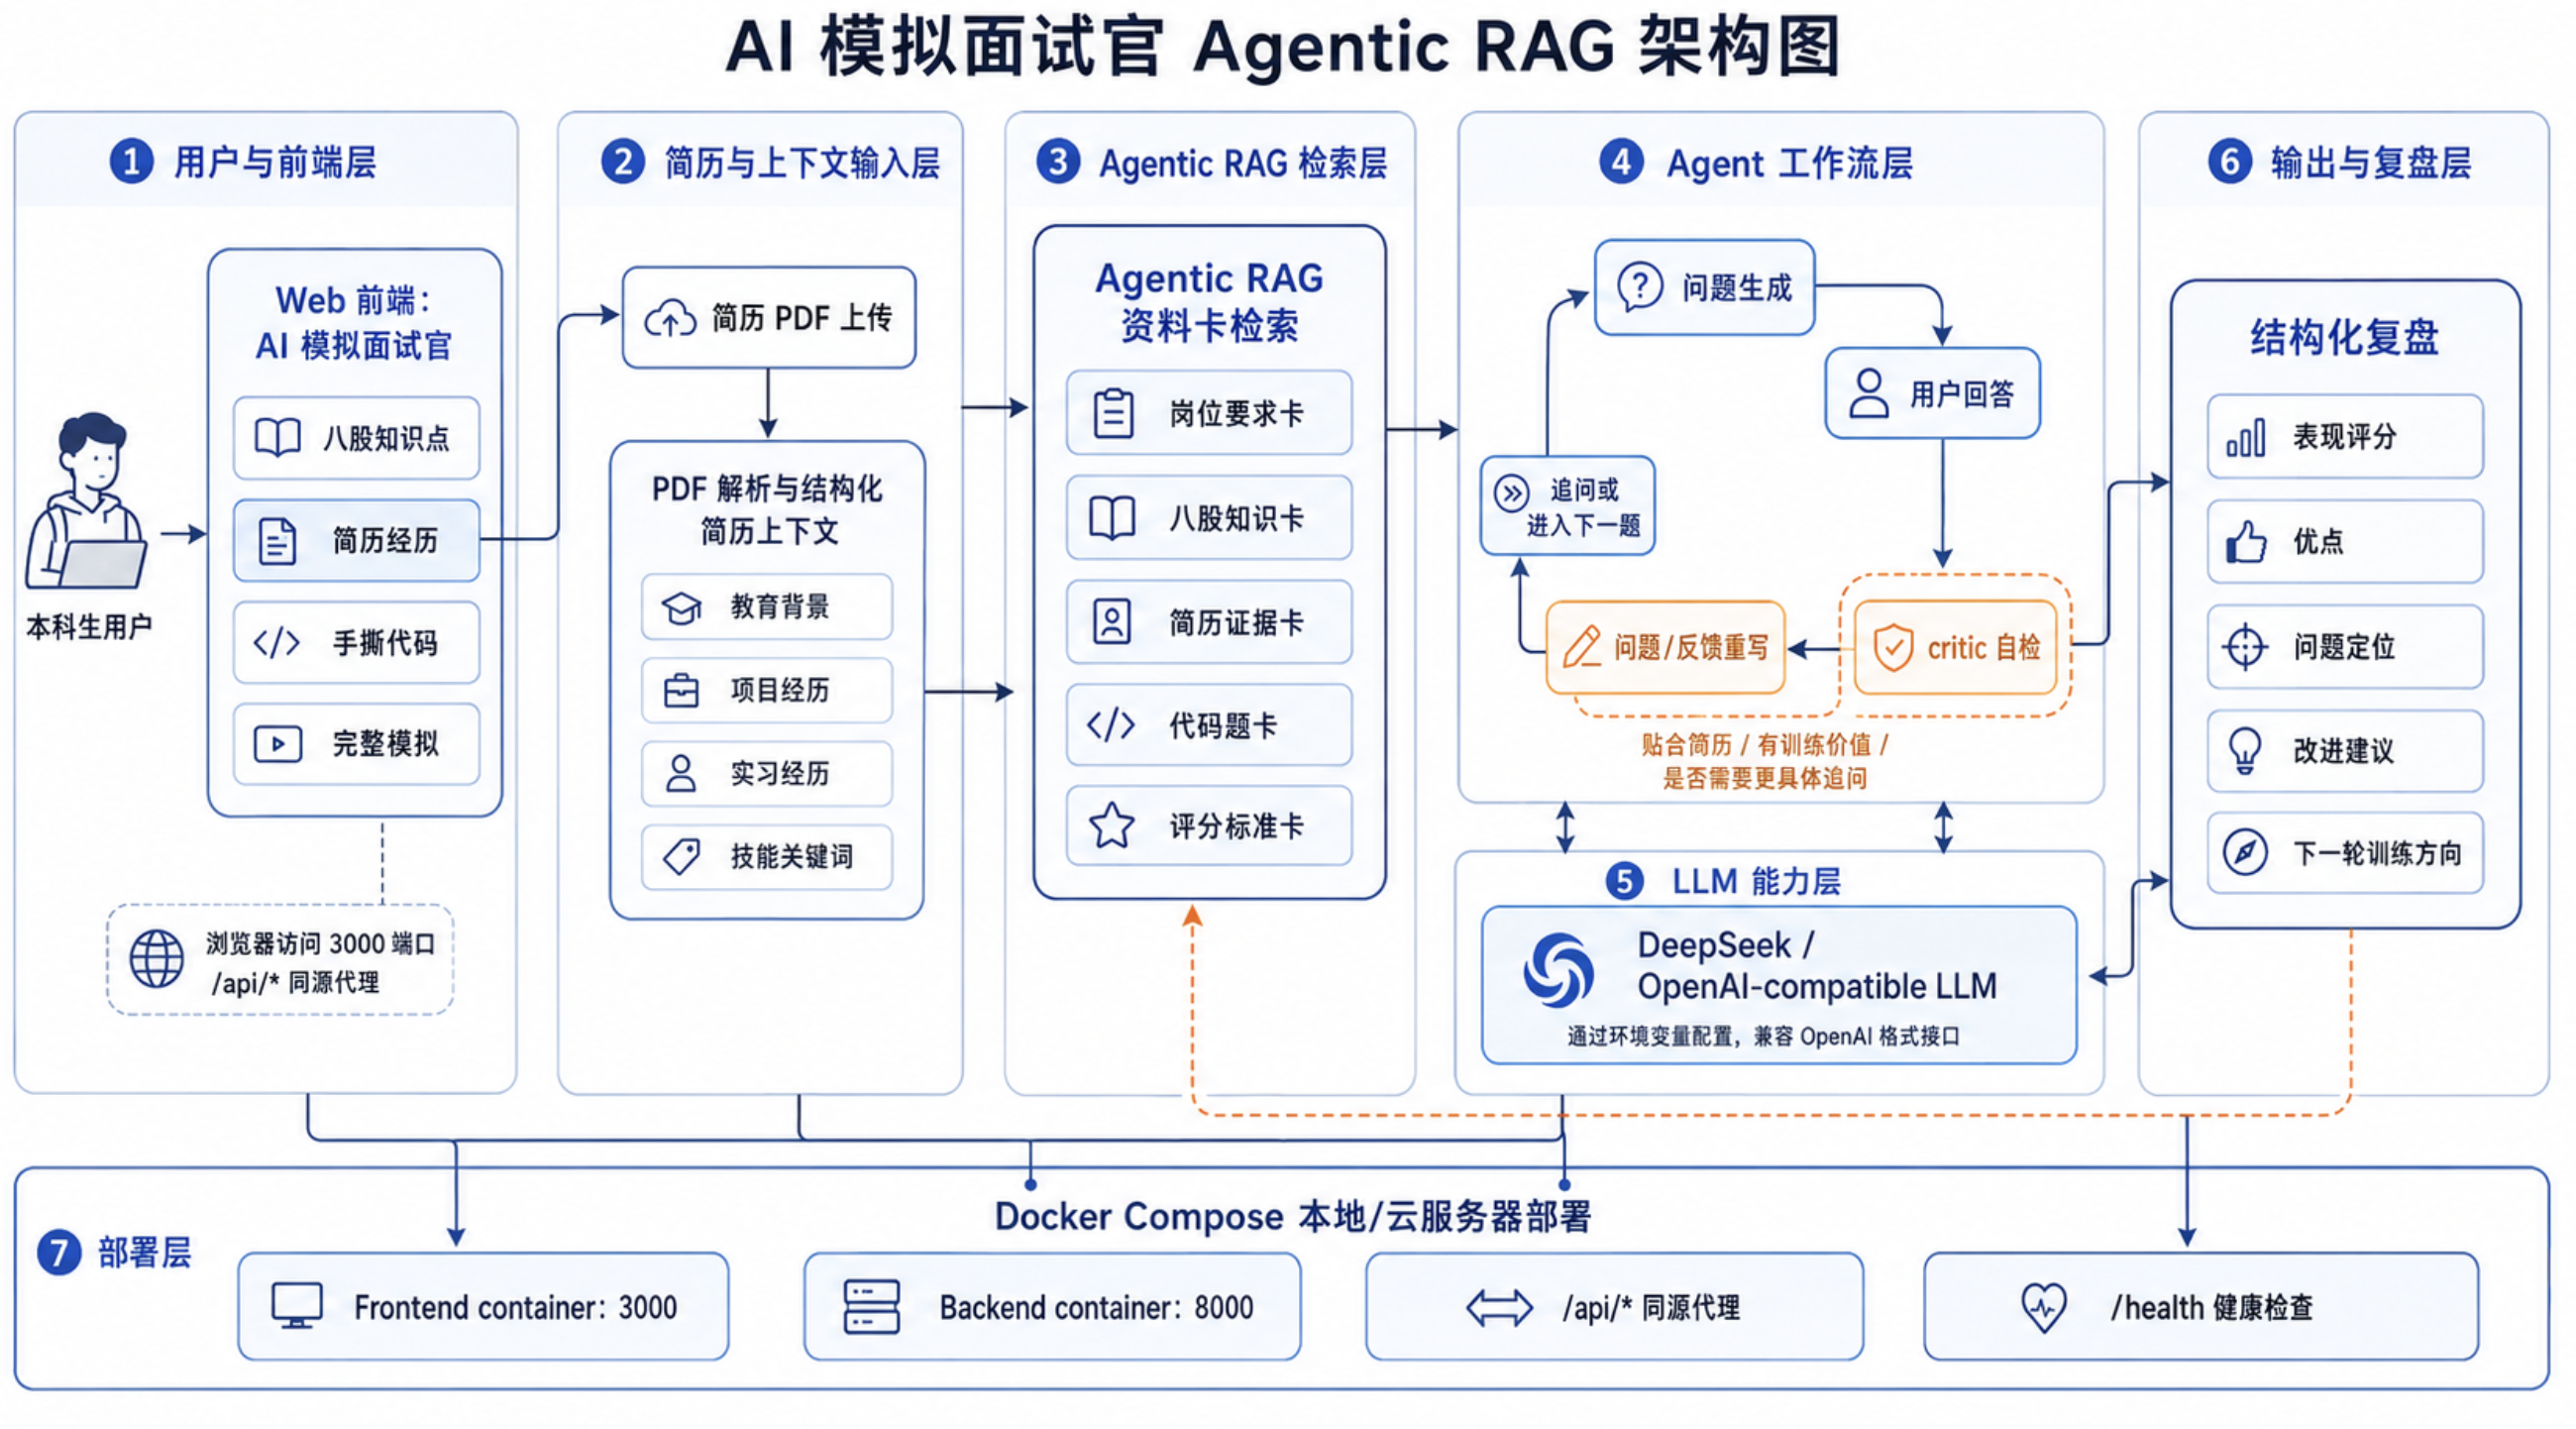
\includegraphics[width=0.93\linewidth,height=4.2cm,keepaspectratio]{fig/image.png}
\end{center}

\sectionline{4. 商业目标、指标与行动计划}
\begin{minipage}[t]{0.48\linewidth}
\small
\textbf{MVP KPI}
\begin{itemize}
  \item 激活率：上传/加载简历后开始第一轮训练。
  \item 完成率：完成至少 3 轮并生成复盘。
  \item 复练率：24 小时内回到同一挂点训练。
  \item 质量评分：问题贴合度、复盘可执行性 1--5 分。
\end{itemize}
\textbf{商业路径：}Freemium 起步，付费解锁完整模拟、历史报告、JD 匹配和复练计划；B 端面向高校就业中心、求职社团和训练营提供批量账号与训练看板。
\end{minipage}
\hfill
\begin{minipage}[t]{0.49\linewidth}
\footnotesize
\begin{tabular}{p{0.18\linewidth}p{0.62\linewidth}p{0.12\linewidth}}
\toprule
时间 & 里程碑 & 级别 \\
\midrule
1 周 & JD 匹配、历史训练、资料卡扩充 & P0 \\
2--3 周 & 用户测试、挂点复练、报告优化 & P0/P1 \\
1 月 & 语音压力面、趋势报告、高校试点 & P1 \\
2--3 月 & 题库运营、付费转化、B 端看板 & P2 \\
\bottomrule
\end{tabular}
\vspace{0.25em}

资源需求：产品/增长做访谈和指标看板，全栈做历史记录与权限，LLM 工程维护资料卡、评测集和 rubric。优先级保持“训练价值 > 功能数量 > UI 精致度”。
\end{minipage}

\end{document}
